\chapter{System Architecture and Multimodal Data Modeling}

\section{System Design Objectives and Modeling Scope}
Chapter 1 has described the research content and main contributions of this thesis. On that basis, this chapter focuses on the system-level model rather than restating the technical route. Its purpose is to specify how heterogeneous observations are organized before the dedicated methods in later chapters are introduced. Therefore, the emphasis of this section is placed on design objectives, input assumptions, module boundaries, and common data structures.

\begin{enumerate}
  \item Target-centered organization. The system does not directly concatenate raw signals from different sources. Optical images, electromagnetic records, SAR observations, and historical trajectories are first converted into target-level observations or trajectory fragments. This organization keeps the later fusion process focused on physical entities rather than on isolated sensor records.

  \item Missing-data modeling. Different modalities may provide observations at different times and with different spatial references. The model distinguishes coordinate-known observations, coordinate-missing optical images, absent target states, and unreliable detections. The system records such uncertainty through coordinate status, confidence values, and validity masks.

  \item Scene retrieval and target association. For optical images without coordinates, visual reference retrieval can provide coordinate-known scene candidates, but it cannot directly determine target identity. The system design therefore treats retrieval results as constraints for later association, not as final fusion decisions.

  \item Relation-aware representation. Target identity and behavior cannot always be determined from a single target state. The data model must preserve temporal continuity, spatial neighborhoods, and possible cross-modal correspondences. These relations provide the shared basis for entity-level registration and behavior analysis.
\end{enumerate}

Accordingly, the output of this chapter is a system specification rather than an algorithmic contribution. The following sections define the overall architecture, data-source characteristics, coordinate-missing optical access condition, unified target state, modality-specific trajectory set, fused entity form, and spatiotemporal graph representation. These definitions provide a common notation and data interface for the later method chapters.

\section{Overall System Architecture}
The proposed system is organized into six functional layers: multimodal data input, preprocessing, optical reference retrieval, entity-level fusion, behavior analysis, and result presentation. Each layer corresponds to a different level of information abstraction, from raw observations to interpretable situation outputs.

Fig.~\ref{fig:chapter2-layered-architecture} provides the corresponding layered view. It shows how heterogeneous observations are progressively transformed from raw inputs into target records, reference candidates, fused entities, anomaly evidence, and final situation outputs. The figure also indicates the method layers that are developed in Chapters 3, 4, and 5.

\begin{figure}[htb]
  \centering
  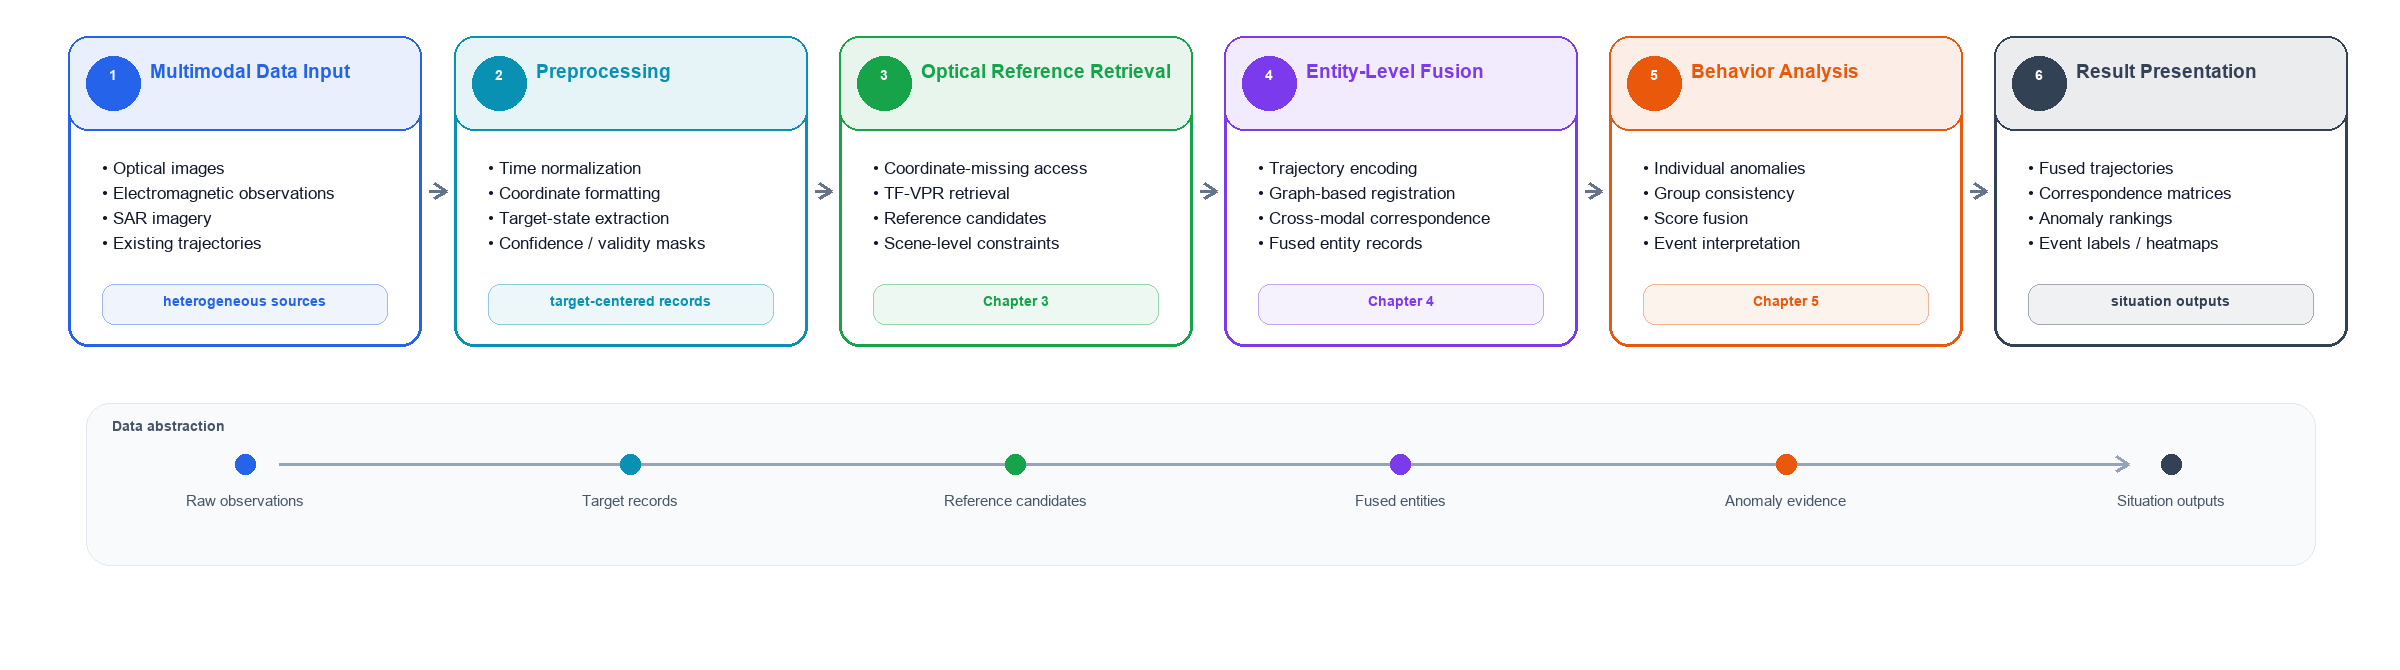
\includegraphics[width=\textwidth]{images/chapter2/chapter2_layered_architecture.png}
  \caption{Layered architecture of the multimodal target fusion and behavior analysis system. Heterogeneous observations are organized through preprocessing, TF-VPR-based optical reference retrieval, entity-level fusion, behavior analysis, and result presentation.}
  \label{fig:chapter2-layered-architecture}
\end{figure}

The multimodal data input layer receives heterogeneous observations. Optical images provide visual appearance, target categories, local image context, and image-plane locations. Electromagnetic observations may provide signal-related or motion-related cues. SAR images provide wide-area sensing under adverse weather or illumination conditions, but their imaging geometry differs from optical imagery. Existing trajectories provide historical target states and temporal continuity. These sources are complementary, but their coordinate systems and feature spaces are not directly compatible.

The preprocessing layer converts raw observations into modality-specific target records. This layer performs time formatting, coordinate normalization, target-state extraction, confidence estimation, missing-value marking, and trajectory organization. Its output is a set of single-modal or partially completed trajectories, rather than the final fused result.

The optical reference retrieval layer handles coordinate-missing optical images. For such images, detected target positions cannot be projected directly into the spatial frame used by other modalities. The system therefore uses TF-VPR to retrieve coordinate-known reference images for each coordinate-missing query. These references provide scene-level constraints for downstream target association.

The entity-level fusion layer estimates whether entities from different modalities correspond to the same physical target. Completed trajectories are first encoded into target-level embeddings. These embeddings are refined through intra-set and cross-set graph interaction, and soft correspondences are then estimated across modality-specific entity sets. Reliable correspondences are used to aggregate trajectory states and modality-specific attributes into fused entity records.

The behavior analysis layer evaluates fused entities. It contains an individual-level detector and a group-level detector. The individual detector measures whether a target's own motion pattern is unusual. The group detector measures whether the target remains consistent with its local group and whether the group undergoes abnormal structural changes. The two sources of evidence are combined into object-level anomaly scores and event decisions.

The result presentation layer converts the system outputs into interpretable records. These records include fused trajectories, cross-modal correspondence matrices, anomaly rankings, event explanations, and situation heatmaps. They support later inspection of both fusion quality and behavior-level situation changes.

After the structural overview in Fig.~\ref{fig:chapter2-layered-architecture}, Table~\ref{tab:chapter2-module-interface} summarizes the interfaces of the main modules. The table describes each module at the system level. Detailed algorithmic designs are presented in Chapters 3, 4, and 5.

\begin{table}[htb]
  \centering
  \caption{Functional interfaces of the main system modules.}
  \label{tab:chapter2-module-interface}
  \setlength{\tabcolsep}{4pt}
  \renewcommand{\arraystretch}{0.95}
  \small
  \begin{tabular}{>{\raggedright\arraybackslash}p{0.20\textwidth}>{\raggedright\arraybackslash}p{0.25\textwidth}>{\raggedright\arraybackslash}p{0.25\textwidth}>{\raggedright\arraybackslash}p{0.22\textwidth}}
    \toprule
    Module & Input & Output & Main function \\
    \midrule
    Multimodal preprocessing & Raw optical, electromagnetic, SAR, and trajectory data & Modality-specific target records & Normalizes format, time, coordinates, attributes, and confidence information \\
    TF-VPR reference retrieval & Coordinate-missing optical image and coordinate-known reference image database & Top-\(k\) reference image candidates & Provides scene-level constraints for optical target association \\
    Target association and trajectory organization & Pixel-level detections and retrieved references & Completed optical trajectory segments & Connects image-plane observations to target or trajectory identifiers \\
    Entity-level registration & Modality-specific trajectory sets & Cross-modal correspondence matrices & Estimates whether entities from different modalities refer to the same physical target \\
    Multimodal fusion & Matched entity groups and correspondence confidence & Fused target records & Aggregates trajectories, attributes, and confidence into unified entities \\
    Behavior analysis & Fused entity trajectories & Anomaly scores, event labels, and heatmaps & Detects individual and group anomalies and supports situation presentation \\
    \bottomrule
  \end{tabular}
\end{table}

\section{Multimodal Data Sources and Feature Analysis}
The system uses several types of input data. Each modality contributes useful information to target understanding, but each also introduces specific uncertainty. Analyzing these properties is necessary before defining the data model.

Optical images provide rich appearance and semantic information. Targets can be described by bounding boxes, centers, local patches, category labels, visual features, and surrounding scene context. Optical data are useful for recognition and visual association. However, they are sensitive to illumination variation, viewpoint change, occlusion, weather, and image quality. Some optical images also lack reliable geographic metadata, which prevents direct comparison with spatial trajectories.

Electromagnetic observation data provide complementary target-related evidence, such as signal characteristics, motion cues, or observation confidence. This modality may be less affected by visual appearance changes. However, it usually has weaker semantic descriptions of target category and local structure. Its feature space may also differ substantially from image-based feature spaces.

SAR imagery provides wide-area and all-weather observation. It can remain informative when optical images are degraded by weather or illumination. However, SAR uses a different imaging mechanism. Target appearance and background structure in SAR images are not directly comparable with optical images. Geometric distortion and speckle noise can further complicate target-level association.

Existing trajectories provide historical target states and temporal continuity. They are important because behavior analysis depends on target evolution over time. Nevertheless, existing trajectories may be incomplete, asynchronous with new observations, or inconsistent with newly detected targets. They may also contain missing segments or identity switches.

These complementary properties motivate target-level multimodal fusion. Optical images provide semantic and appearance cues. Electromagnetic and SAR observations provide additional sensing evidence. Existing trajectories provide temporal context. At the same time, their heterogeneity requires a unified representation and an explicit cross-modal registration mechanism. Table~\ref{tab:chapter2-data-source} summarizes the main properties of the data sources considered in this thesis.

\begin{table}[htb]
  \centering
  \caption{Characteristics of multimodal data sources.}
  \label{tab:chapter2-data-source}
  \small
  \begin{tabular}{p{0.17\textwidth}p{0.25\textwidth}p{0.25\textwidth}p{0.25\textwidth}}
    \toprule
    Data source & Main information & Advantage & Limitation \\
    \midrule
    Optical imagery & Appearance, category, image-plane position, scene context & Rich visual semantics and intuitive target description & Sensitive to illumination, viewpoint, occlusion, weather, and missing geographic metadata \\
    Electromagnetic observation & Signal-related attributes, motion-related cues, observation confidence & Provides complementary non-visual evidence & Weak visual semantics and modality-specific feature space \\
    SAR imagery & Wide-area target response and spatial structure & All-weather and wide-area observation capability & Different imaging geometry, speckle noise, and difficult optical-SAR comparison \\
    Existing trajectories & Historical positions, velocities, and target identities & Provides temporal continuity and prior target context & May be incomplete, asynchronous, or inconsistent with new observations \\
    \bottomrule
  \end{tabular}
\end{table}

From a system-design perspective, these data sources should not be fused directly at the raw-signal level. Their raw forms are too different, and direct concatenation would obscure modality-specific reliability. This thesis therefore adopts target-level fusion. Each modality is first converted into target observations or trajectory fragments. Fusion is then performed after target-level representations have been established.

\section{Existing Trajectories and Coordinate-Missing Optical Images}
The data condition considered in this thesis includes both coordinate-known and coordinate-missing observations. For coordinate-known optical images and other spatially referenced observations, target detections can be projected into a common coordinate frame and linked with existing trajectories through spatial and temporal constraints. By contrast, coordinate-missing optical images provide only pixel-level target observations. These observations cannot be directly compared with trajectories from electromagnetic, SAR, or historical sources. Therefore, an additional access mechanism is required to connect image-plane observations to the existing trajectory system.

As illustrated in Fig.~\ref{fig:chapter2-optical-access}, the access mechanism separates scene-level reference retrieval from target-level association. TF-VPR retrieves coordinate-known reference candidates for a coordinate-missing query and thereby narrows the candidate search space. The downstream association module then uses the pixel-level detections, retrieved references, and existing trajectory records to estimate target-level correspondence and generate an optical trajectory segment or association record.

\begin{figure}[htb]
  \centering
  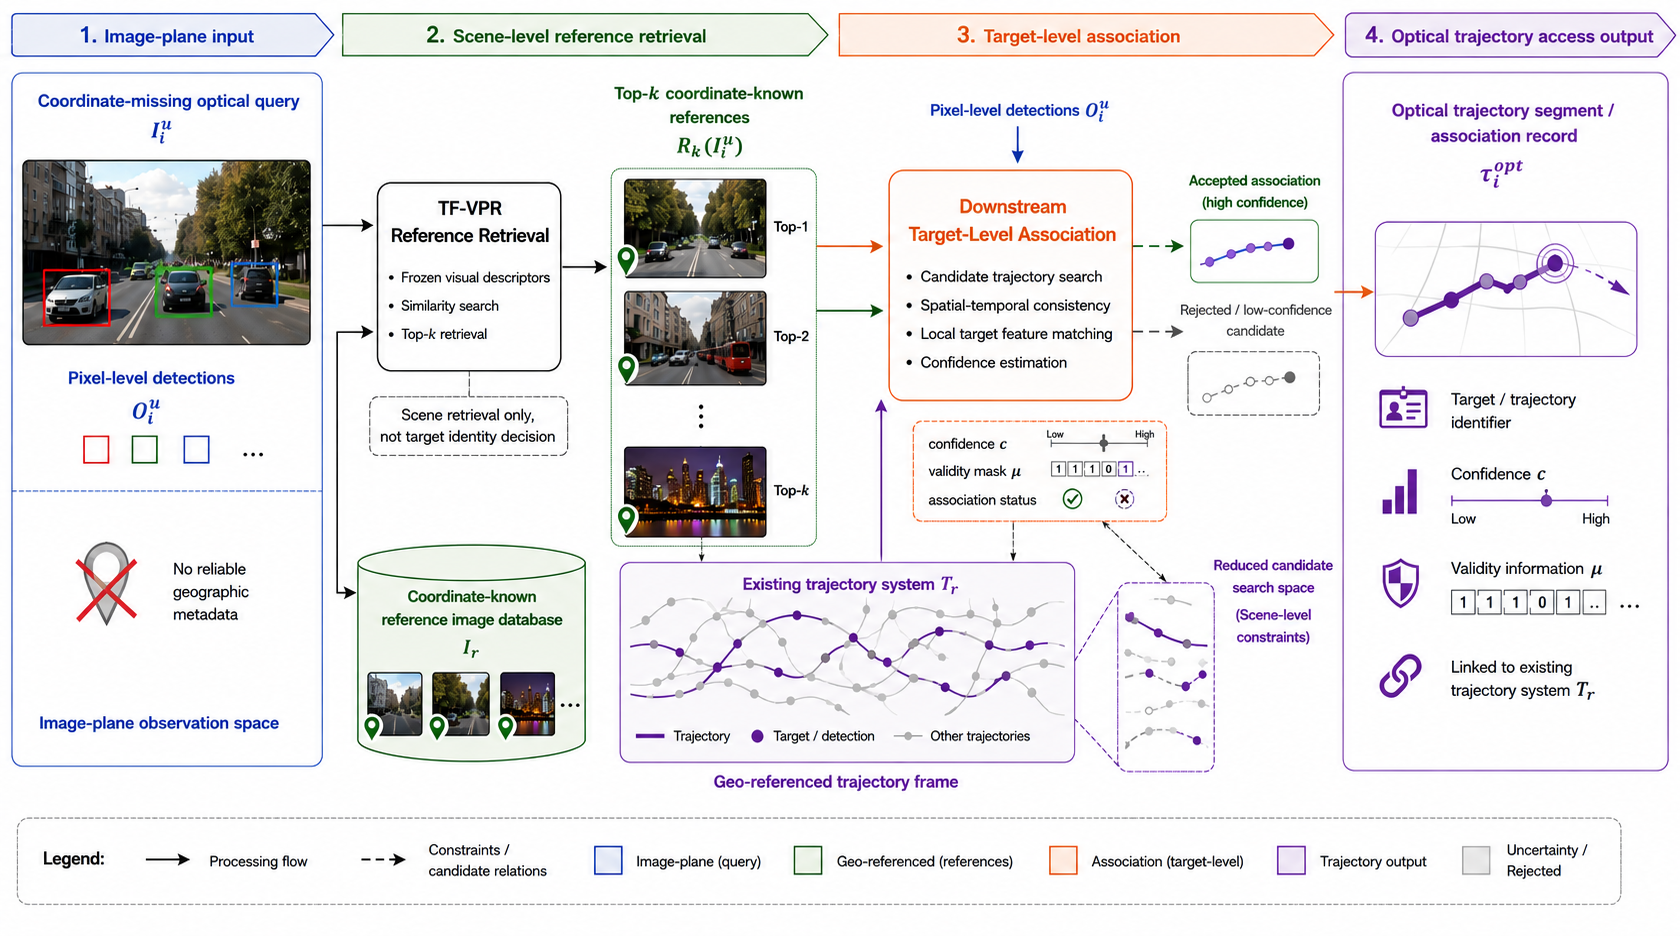
\includegraphics[width=\textwidth,height=0.42\textheight,keepaspectratio]{images/chapter2/coordinate_missing_optical_access.png}
  \caption{Coordinate-missing optical access mechanism. TF-VPR provides scene-level coordinate-known reference candidates for coordinate-missing optical queries, while the downstream association module uses these candidates to constrain target-level trajectory association and output an optical trajectory segment or association record.}
  \label{fig:chapter2-optical-access}
\end{figure}

Consistent with the notation in Fig.~\ref{fig:chapter2-optical-access}, let \(I_u=\{I^u_1,I^u_2,\ldots,I^u_{N_u}\}\) denote the set of coordinate-missing optical images, where \(N_u\) is the number of such images. Let \(I_r=\{I^r_1,I^r_2,\ldots,I^r_{N_r}\}\) denote the coordinate-known optical reference database, where \(N_r\) is the number of reference images. For the \(i\)-th coordinate-missing image \(I^u_i\), a target detector can provide pixel-level observations
\begin{equation}
  O^u_i = \{o^u_{i,1},o^u_{i,2},\ldots,o^u_{i,n_i}\},
\end{equation}
where \(O^u_i\) is the observation set of image \(I^u_i\), \(o^u_{i,l}\) is the \(l\)-th detected target observation in that image, and \(n_i\) is the number of detected target observations. Each observation may include a bounding box, a target center, a category label, and a local target feature. Without a geographic reference, \(O^u_i\) cannot be directly mapped into the spatial trajectory set.

The system therefore first performs image-level reference retrieval:
\begin{equation}
  \mathcal{R}_k(I^u_i)
  =
  \operatorname{TopK}_{I^r_j\in I_r}
  \operatorname{sim}\big(g(I^u_i),g(I^r_j)\big),
\end{equation}
where \(g(\cdot)\) denotes the image descriptor generated by TF-VPR. The function \(\operatorname{sim}(\cdot,\cdot)\) denotes descriptor similarity. The retrieved set \(\mathcal{R}_k(I^u_i)\) contains the top-\(k\) coordinate-known references that are visually related to the query.
Here, \(k\) is the number of retained reference candidates, and \(\operatorname{TopK}_{I^r_j\in I_r}\) returns the \(k\) reference images with the highest similarity scores among all \(I^r_j\) in \(I_r\).

The retrieval result is a scene-level constraint, not a final target-level association. A high image similarity score indicates that the query and reference images are visually related. It does not prove that a detected target in the query corresponds to a specific target in the reference data. As shown by the constraint path in Fig.~\ref{fig:chapter2-optical-access}, the retrieved references are therefore used to reduce the search space for downstream association. The target association module then compares pixel-level detections, local target features, temporal consistency, and candidate trajectory states within this constrained set.

After target association, coordinate-missing optical observations can be converted into optical trajectory segments or association records:
\begin{equation}
  \tau^{\mathrm{opt}}_a
  =
  \{x^{\mathrm{opt}}_{a,t_1},x^{\mathrm{opt}}_{a,t_2},\ldots,x^{\mathrm{opt}}_{a,t_{L_a}}\}.
\end{equation}
Here, \(a\) indexes an associated optical target, \(t_1,\ldots,t_{L_a}\) are the time stamps of the segment, \(L_a\) is the segment length, and \(x^{\mathrm{opt}}_{a,t}\) is the optical target state at time \(t\). This output corresponds to the optical trajectory access result in Fig.~\ref{fig:chapter2-optical-access}. These segments do not need to be perfect before entering the fusion stage. They provide target-level evidence with explicit confidence and validity information. Chapter 4 then combines this optical evidence with other modalities and suppresses unreliable correspondences through relation-aware matching.

This design has two advantages. First, it avoids assuming that every optical image has accurate geographic metadata. Second, it separates image-level scene retrieval from target-level identity association. TF-VPR locates candidate reference scenes without additional scene-specific training. The downstream association module then focuses on target correspondence within a smaller candidate space.

\section{Multimodal Data Preprocessing and Unified Representation}
Before multimodal fusion, observations from different sources must be converted into a common target-centered format. The purpose of preprocessing is not to remove modality differences. Instead, it organizes heterogeneous information so that it can be compared, registered, and fused at the entity level.

The preprocessing stage contains four basic operations. First, time stamps are normalized to a common temporal reference. When modalities have different sampling rates, each observation is assigned to a discrete time index or interval. Second, spatial information is formatted consistently. Coordinate-known observations are represented in the spatial frame when possible. Coordinate-missing optical observations remain in the image plane until they are connected to reference trajectories. Third, modality-specific attributes are extracted and stored without forcing them into identical feature dimensions. Fourth, missing observations and uncertainty are recorded through masks and confidence scores.

For modality \(m\), the target state of entity \(i\) at time \(t\) is represented as
\begin{equation}
  x_{i,t}^{(m)}
  =
  \big[
  p_{i,t}^{(m)},\,
  v_{i,t}^{(m)},\,
  f_{i,t}^{(m)},\,
  c_{i,t}^{(m)},\,
  \mu_{i,t}^{(m)}
  \big],
  \label{eq:chapter2-target-state}
\end{equation}
where \(p_{i,t}^{(m)}\) denotes position information, \(v_{i,t}^{(m)}\) denotes motion information, and \(f_{i,t}^{(m)}\) denotes modality-specific attributes. The term \(c_{i,t}^{(m)}\) denotes observation confidence, and \(\mu_{i,t}^{(m)}\) denotes the validity mask.

The position term \(p_{i,t}^{(m)}\) may have different meanings before and after reference connection. For spatially referenced observations, it represents a position in the common coordinate frame. For coordinate-missing optical images before association, it may represent an image-plane center or bounding-box position. After TF-VPR-based retrieval and target association, optical observations can be linked to candidate trajectory identifiers and used in the fusion stage.

The motion term \(v_{i,t}^{(m)}\) describes target dynamics, such as velocity, displacement, or direction. It can be computed from consecutive positions when raw velocity is unavailable. The attribute term \(f_{i,t}^{(m)}\) preserves modality-specific information, including optical appearance features, electromagnetic attributes, SAR response descriptors, or historical trajectory descriptors. The confidence term \(c_{i,t}^{(m)}\) records observation reliability. The mask term \(\mu_{i,t}^{(m)}\in\{0,1\}\) indicates whether modality \(m\) provides a valid observation for target \(i\) at time \(t\).

Based on Eq.~\eqref{eq:chapter2-target-state}, a modality-specific trajectory is written as
\begin{equation}
  \tau_i^{(m)}
  =
  \{x_{i,t_1}^{(m)},x_{i,t_2}^{(m)},\ldots,x_{i,t_L}^{(m)}\},
\end{equation}
and the trajectory set of modality \(m\) is written as
\begin{equation}
  \mathcal{T}^{(m)}
  =
  \{\tau_1^{(m)},\tau_2^{(m)},\ldots,\tau_{N_m}^{(m)}\}.
\end{equation}
Here, \(\tau_i^{(m)}\) denotes the trajectory of entity \(i\) in modality \(m\), \(t_1,t_2,\ldots,t_L\) denote the ordered time stamps of the trajectory, and \(L\) denotes the number of states in the trajectory. The set \(\mathcal{T}^{(m)}\) contains all modality-\(m\) trajectories, and \(N_m\) denotes the number of trajectories in this modality.

This representation has three functions. First, it allows all modalities to share a target-level structure while preserving modality-specific attributes. Second, it avoids treating missing data as ordinary numerical values. Missing observations are explicitly marked by \(\mu_{i,t}^{(m)}\). Third, it provides the input interface for entity-level registration in Chapter 4 and behavior analysis in Chapter 5.

After cross-modal registration and fusion, the final fused entity can be represented as
\begin{equation}
  e_j = \{T_j,F_j,C_j\},
\end{equation}
where \(e_j\) denotes the \(j\)-th fused entity, \(T_j\) denotes its fused trajectory component, \(F_j\) denotes its fused multimodal attribute component, and \(C_j\) denotes its confidence information. Chapter 4 describes how this fused representation is generated. In this chapter, the key point is that Eq.~\eqref{eq:chapter2-target-state} defines the data basis from which fused entities are constructed.

\section{Spatiotemporal Graph Construction}
Target fusion and behavior analysis both require relational information. A target cannot always be identified by local attributes alone, especially when different modalities use different feature spaces. Similarly, abnormal behavior cannot always be detected from one trajectory alone. Many abnormal events are defined by the relation between a target and its surrounding group. The system therefore organizes preprocessed target records as spatiotemporal graphs.

At time \(t\), visible target states are treated as graph nodes:
\begin{equation}
  \mathcal{V}_t
  =
  \{z_{i,t}\mid \mu_{i,t}=1\}.
\end{equation}
Here, \(z_{i,t}\) denotes the graph node corresponding to target \(i\) at time \(t\), and \(\mu_{i,t}\) denotes the validity mask of the corresponding target state. When the graph is built for a specific modality, the superscript \((m)\) in \(\mu_{i,t}^{(m)}\) is omitted for readability. Each node stores the target-centered state in Eq.~\eqref{eq:chapter2-target-state}, or a feature embedding derived from that state. The graph contains three types of edges: temporal edges, spatial edges, and cross-modal candidate edges.

Temporal edges connect observations or states that belong to the same target across adjacent time steps:
\begin{equation}
  \mathcal{E}^{\mathrm{time}}
  =
  \{(z_{i,t},z_{i,t+1})\mid z_{i,t}\in\mathcal{V}_t,\ z_{i,t+1}\in\mathcal{V}_{t+1}\}.
\end{equation}
These edges preserve trajectory continuity and support later motion modeling. In this formula, the same target index \(i\) indicates that the two nodes belong to the same target at adjacent time steps.

Spatial edges connect targets that are close in position, motion, or local context within the same time step:
\begin{equation}
  \mathcal{E}^{\mathrm{space}}_t
  =
  \{(z_{i,t},z_{j,t})\mid j\in\mathcal{N}_K(i,t)\},
\end{equation}
where \(\mathcal{N}_K(i,t)\) denotes the \(K\)-nearest neighbors of target \(i\) at time \(t\), \(j\) denotes a neighboring target index, and \(K\) is the preset neighborhood size. The neighborhood can be defined by spatial distance, motion similarity, category consistency, confidence, or a combination of these factors. These edges provide the structural basis for group behavior modeling in Chapter 5.

Cross-modal candidate edges connect entities from different modalities when they may correspond to the same physical target:
\begin{equation}
  \mathcal{E}^{\mathrm{cross}}
  =
  \{(\tau_i^{(m)},\tau_j^{(n)})\mid m\neq n,\ \operatorname{comp}(\tau_i^{(m)},\tau_j^{(n)})>\delta\},
\end{equation}
where \(m\) and \(n\) are two different modality indices, \(i\) and \(j\) are trajectory indices within the corresponding modalities, and \(\operatorname{comp}(\cdot,\cdot)\) denotes a compatibility score based on temporal overlap, spatial consistency, attribute similarity, and confidence. The threshold \(\delta\) defines the candidate relation set. These edges do not impose final identity decisions. They only define plausible cross-modal relations to be refined by the registration method in Chapter 4.

The graph representation can be written as
\begin{equation}
  \mathcal{G}
  =
  (\mathcal{V},\mathcal{E}^{\mathrm{time}},\mathcal{E}^{\mathrm{space}},\mathcal{E}^{\mathrm{cross}}).
\end{equation}
In this representation, \(\mathcal{G}\) denotes the spatiotemporal graph, \(\mathcal{V}=\bigcup_t\mathcal{V}_t\) denotes the complete node set over all time steps, and \(\mathcal{E}^{\mathrm{space}}=\bigcup_t\mathcal{E}^{\mathrm{space}}_t\) denotes all spatial edges. Temporal edges describe target evolution, spatial edges describe target interaction, and cross-modal edges describe possible identity correspondences.

The graph is used differently in later chapters. In Chapter 4, graph interaction supports entity-level registration. Modality-specific entity sets are refined through intra-set and cross-set interaction, and the resulting features are used to estimate soft correspondence matrices. In Chapter 5, the graph supports behavior analysis. Spatial and temporal edges describe group structure and motion evolution, while abnormal behavior is detected from prediction errors and interpretable group-event indicators.

The spatiotemporal graph defined here is therefore a system-level data structure rather than a single fixed algorithm. It provides a common relational representation for multimodal fusion and behavior understanding.

\section{Chapter Summary}
This chapter presented the system architecture and data modeling strategy of the proposed multimodal target fusion and behavior analysis framework. The system was organized as a staged pipeline from heterogeneous data input to fused entity representation and behavior analysis output. The chapter also clarified the role of multimodal preprocessing, TF-VPR-based optical reference retrieval, target association, entity-level registration, multimodal fusion, and behavior analysis.

The chapter analyzed the characteristics of optical, electromagnetic, SAR, and existing trajectory data. Their complementary advantages motivate multimodal fusion, but their differences in coordinate systems, sampling rates, feature spaces, and uncertainty require a unified target-level representation. For coordinate-missing optical images, the chapter explained why image-level reference retrieval is needed before target-level association, and why TF-VPR is used as the retrieval module.

Finally, this chapter defined a target-centered state representation and a spatiotemporal graph structure for temporal continuity, spatial neighborhoods, and cross-modal candidate correspondences. These definitions provide the data interface for Chapter 3's TF-VPR retrieval, Chapter 4's entity-level fusion, and Chapter 5's behavior analysis.
